\section{Outils de développement}
Cette partie est réservée aux différents outils de travail utilisés durant les différentes phases du projet.

\begin{figure}[h!]  
 \centering
    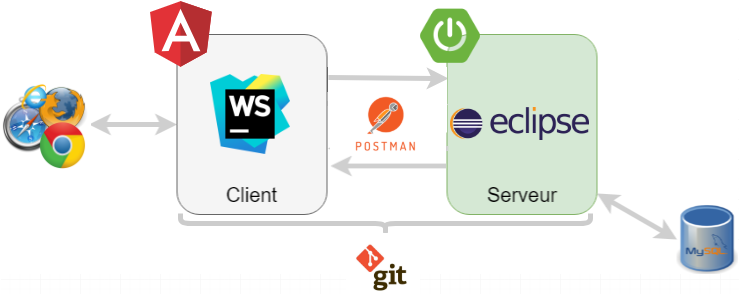
\includegraphics[width=1\textwidth]{chapitre5/Figures/outils.png}
  \caption{Outils utilisés}
\end{figure}

La liste non exhaustive suivante donne une idée sur notre environnement de travail :
\begin{itemize}[label=\textbullet]
  \item Astah permettant la modélisation UML
  \item Eclipse est l'IDE utilisé pour développer le Back-end
  \item Git est le logiciel consacré à la gestion du code source
  \item MySQL a pour but la sauvegarde et la restitution des données
  \item Postman est l'outil choisi pour tester les API REST
  \item WebStorm est l'IDE utilisé pour développer le Front-end
\end{itemize}

Les outils susmentionnés sont décrits en détails dans l'Annexe C.